Tässä luvussa käsitellään puhtaasti murtolukujen laskutekniikkaa, ja seuraavassa luvussa harjoitellaan, miten nämä laskutoimitukset liittyvät sovelluksiin.

\subsection{Murtolukuesitys}
Rationaaliluvun esitystä kokonaislukujen osamääränä $\frac{a}{b}$ kutsutaan \termi{murtoluku}{murtoluvuksi}. Luku $a$ on murtoluvun \termi{osoittaja}{osoittaja} ja luku $b$ on \termi{nimittäjä}{nimittäjä}. Nimittäjä on aina erisuuri kuin nolla ($b\neq0 $). Määritelmän mukaan kaikki rationaaliluvut voidaan esittää murtolukuina. Usein rationaaliluvut voidaan esittää myös desimaaliesityksen avulla. %LAUSUMINEN! ``kolme kahdesosaa''

Rationaalilukuja esitetään toisinaan myös \termi{sekamurtoluku}{sekamurtolukuina} eli lyhyemminsekalukuina. Sekalukuesityksessä luku esitetään summana kokonaisosasta ja murto-osasta (yleensä luku nollan ja yhden väliltä), mutta yhteenlaskumerkki jätetään merkitsemättä. Esimerkiksi sekaluku $3\frac{1}{4}$ tarkoittaa lukua $3 + \frac{1}{4}$, jonka voi esittää murtolukuna $\frac{13}{4}$. Jos luku on negatiivinen, miinusmerkki merkitään koko sekaluvun eteen, siis $-6\frac{4}{5}$ tarkoittaa lukua $-(6 + \frac{4}{5})$. Merkintä saattaa aiheuttaa sekaannusta, sillä $3\frac{5}{6}$ saattaisi myös viitata tuloon $3\cdot \frac{5}{6}$. Sekalukumerkintää käytetään vain tunnetuilla lukuarvoilla, siis $a\frac{b}{c}$ tarkoittaa aina tuloa $a\cdot \frac{b}{c}$. 

\begin{esimerkki}
        Rationaaliluvulla $\frac{5}{4}$ on kolme erilaista esitystapaa: murtolukuesitys, sekalukuesitys ja desimaaliesitys.
        \[\frac{5}{4} = 1\frac{1}{4}=1,25 \]
\end{esimerkki} %nimityksen esittely pois esimerkistä!

Murtolukujen laskutoimituksia varten sekaluvut kannattaa usein muuttaa murtolukuesitykseksi. 
\newpage

Jos kahdella murtoluvulla on sama nimittäjä, niitä sanotaan \termi{samannimisyys}{samannimisiksi}. %yhdyssana\ldots? JA TARKISTA MURTOLUKU, RATIONAALUKU, MURTOLUKUMUOTO, MURTOLUKUESITYS -KOHERENSSI!!!

\begin{esimerkki}
Luvut $\frac15$, $\frac75$ ja $-\frac{25}{5}$ ovat keskenään samannimisiä. Luvut $\frac23$ ja $\frac57$ eivät ole samannimisiä.
\end{esimerkki}

Samannimisten murtolukujen vertailu on helppoa. Kun kaksi murtolukua esittää samankokoisia osia eli nimittäjät ovat samat, nähdään lukujen keskinäinen suuruus suoraan osoittajista. (Tarvittaessa huomioidaan myös mahdollinen negatiivisuus.)

%esimerkki samannimisten murtolukujen vertailusta
%Yleisemmin pätee: jos $a>0$, niin $\frac{b}{a} < \frac{c}{a}$ täsmälleen silloin kun $b<c$.

Jos käsiteltävät murtoluvut eivät jo valmiiksi ole samannimisiä, ne voidaan aina vertailua tai muuta käsittelyä varten muuttaa samannimisiksi \termi{laventaminen}{laventamalla} tai \termi{supistaminen}{supistamalla} %check, käytetään termiympäristöä uudelleen heti :/

\laatikko[Laventaminen ja supistaminen]{
	Murtoluvun arvo pysyy samana, kun sekä osoittajassa että nimittäjässä oleva luku kerrotaan (\termi{laventaminen}{lavennetaan}) samalla luvulla. Vastaavasti, osoittaja ja nimittäjä voidaan jakaa (\termi{supistaminen}{supistaa}) samalla luvulla, jos jako menee tasan.
	\[ \text{laventaminen}\]
	\[ \longrightarrow\]
% \FIXME Nuoliviritys toimisi, mutta rivivälit kaipaavat muokkausta (laventaminen ja nuoli lähemmäs toisiaan). 
	 \[
	 \frac{a}{b} = \frac{ca}{cb}
	 \]
	 
 	\[ \longleftarrow\]
 	\[ \text{supistaminen}\]
 	
	missä $b \neq 0$ ja $c \neq 0$.
}

Laventamisen mahdollistaa se, että jokainen luku $c(\neq0)$ voidaan esittää muodossa $\frac{c}{c}=1$. Kun mielivaltaista lukua kerrotaan luvulla $1$, luvun arvo ei muutu. Huomaa, että murtoluvun laventaminen ei tarkoita samaa kuin murtoluvun kertominen.

Koska murtolukuesitystä voidaan laventaa millä tahansa (nollasta eriävällä) kokonaisluvulla, jokaisella murtoluvulla on monta esitystapaa; esimerkiksi $\frac{1}{2}=\frac{3}{6}$. Konkreettisemmin voidaan ajatella, että puolikas pizza ei vähene vaikka molemmat puolikkaat jaetaan edelleen kolmeen osaan.

\laatikko[Samannimiseksi laventaminen ja supistaminen]{
Mitä tahansa kahta murtolukua voidaan vertailla laventamalla (tai supistamalla) ne samannimisiksi siten, että yhteinen nimittäjä on positiivinen, ja sitten vertaamalla osoittajia.
}

%esimerkki: aseta suuruusjärejstykseen ja kumpi on suurempi ja näytä, että yhtä suuret
%esimerkki: miten jono jatkuu... esitä yleinen muoto :)

\subsection{Murtolukujen yhteen- ja vähennyslasku}

\laatikko[Murtolukujen yhteenlasku, samat nimittäjät]{
    Jos murtolukujen nimittäjät ovat samat, voidaan murtoluvut laskea yhteen laskemalla osoittajat yhteen. %PERUSTELU: PERUSTUU OSITTELULAKIIN
    \[
    \frac{a}{c} + \frac{b}{c} = \frac{a+b}{c}
    \], missä $c \neq 0$
}

Jos yhteenlaskettavilla murtoluvuilla on eri nimittäjät, murtoluvut lavennetaan ensin samannimisiksi ja sitten osoittajat lasketaan yhteen. Jos siis $\frac{a}{b}$ ja $\frac{c}{d}$ ovat murtolukuja (missä $b \neq 0$ ja $d \neq 0$), lasketaan

\laatikko[Murtolukujen yhteenlasku, eri nimittäjät]{
    \[
    \frac{a}{b} + \frac{c}{d} = \frac{ad}{bd} + \frac{bc}{bd} = \frac{ad+bc}{bd}
    \]
    Tässä $\frac{a}{b}$ lavennetaan luvulla $d$ ja $\frac{c}{d}$ lavennetaan luvulla $b$. Nyt saadaan kaksi samannimistä murtolukua, joiden kummankin nimittäjäksi tulee yhteenlaskettavien nimittäjien tulo $bd$.
 }    
 
Yllä esitetty menettely, missä murtoluvut on lavennettu toistensa nimittäjillä toimii aina, mutta toisinaan pelkästään toisen murtoluvun laventaminen tai supistaminen riittää.

\begin{esimerkki}
        Laske
        \[
        \frac{1}{2} + \frac{1}{6} + \frac{2}{6}.
        \]
        
        \begin{esimratk}
        Lavennetaan nimittäjät samannimisiksi ja lasketaan osoittajat yhteen.
        %lisätäänkö lavennusmerkki? teknisesti hankala? käytetäänkö maailmalla? opiskelijoille kuitenkin tuttu
        %tai sitten voisi sanallisesti kertoa, millä lavennetaan.
        \begin{align*}
            \frac{1}{2} + \frac{1}{6} + \frac{2}{6} &=\frac{3\cdot 1}{3\cdot 2} + \frac{1}{6} + \frac{2}{6}\\
            										&=\frac{3}{6} + \frac{1}{6} + \frac{2}{6}\\
           											&= \frac{3+1+2}{6}\\
           											&= \frac{6}{6} = 1.
        \end{align*}
        \end{esimratk}
    \end{esimerkki}
    
\begin{esimerkki}

$ \frac{1}{6} + \frac{3}{2} = \frac{1}{2\cdot 3} + \frac{3}{2} = \frac{1}{2 \cdot 3} + \frac{3 \cdot 3}{2 \cdot 3} = \frac{1}{6} + \frac{9}{6} = \frac{10}{6} = \frac{\cancel{2} \cdot 5}{\cancel{2} \cdot 3} = \frac{5}{3}$

\end{esimerkki}    
    
    Kaikki rationaaliluvut voidaan esittää murtolukumuodossa, mutta myöskokonaisluvut voidaan esittää murtolukuina asettamalla murtoluvun nimittäjäksi yksi. Tätä voidaan käyttää, kun lasketaan yhteen kokonaislukuja ja murtolukuja.
    
    \begin{esimerkki}
        Laske\[ 2 + \frac{1}{3}.\]
                \begin{esimratk}
        Kirjoitetaan lausekkeen kokonaisluku $2$ murtolukuna, minkä jälkeen murtoluvut voidaan laventaa samannimisiksi ja laskea yhteen:
        \begin{align*}
           2 + \frac{1}{3} &= \frac{2}{1} + \frac{1}{3}  \\ 
	   &= \frac{3 \cdot 2}{3 \cdot 1} + \frac{1}{3} \\ 
	   &= \frac{6+1}{3} \\ 
	   &= \frac{7}{3}.
        \end{align*}
                \end{esimratk}
    \end{esimerkki}
    
Murtolukujen vähennyslasku toimii periaatteessa samalla tavalla kuin yhteenlaskukin (vähennyslasku määriteltiin vastaluvun lisäämisenä). Ensin lavennetaan samannimisiksi, sitten suoritetaan vähennyslasku osoittajassa.

%         Murtolukujen nimittäjillä ei ole yhteisiä tekijöitä. Luvut voisi lavetaan kerralla samannimisiksi, mutta voimme käsitellä myös kahta murtolukua kerrallaan. TÄMÄKIN PUUTTUU!


%ei-niin-pitkälle menevä esimerkki vähennyslaskusta
 %selitä, miksi tuo toimii: koska kertolaskun vaihdannaisuus %SEKALUKU PITÄÄ SELITTÄÄ PAREMMIN! ja antaa esimerkkejä!!!
%lisätäänkö lavennusmerkki sievennystehtäviin?
\newpage
\begin{esimerkki}
        Laske \[2\frac{2}{3} - \frac{3}{7}\] ja anna vastaus sekamurtolukuna.
        
        \begin{esimratk}
%tarkista, ovatko nämä selitykset oikeilla riveillä
        \begin{align*}
            2\frac{2}{3} - \frac{3}{7}&=2+\frac{2}{3} - \frac{3}{7} & \text{sekalukuesitys murtoluvuksi}\\
            &=\frac{2}{1}+\frac{2}{3} - \frac{3}{7}\\
            &=\frac{2\cdot3}{1\cdot3}+\frac{2}{3}-\frac{3}{7}\\
            &=\frac{6}{3}+\frac{2}{3}-\frac{3}{7}\\
            &=\frac{6+2}{3} - \frac{3}{7} \\
            &=\frac{8}{3} - \frac{3}{7}\\
            &=\frac{8\cdot7}{3\cdot7} - \frac{3\cdot3}{7\cdot3}\\
            &=\frac{56}{21} - \frac{9}{21}\\
            &=\frac{56-9}{21}\\
            &=\frac{47}{21}\\
            &=\frac{42+5}{21}\\ 
            &=\frac{2\cdot21+5}{21}\\ %selitys
            &=\frac{2\cdot21}{21}+\frac{5}{21}\\ %selitys
            &=\frac{2}{1}+\frac{5}{21}\\
            &=2+\frac{5}{21}\\
            &=2\frac{5}{21}\\
        \end{align*}
        
        (Koska vastaus pyydettiin sekamurtolukuna, ei kokonaisosaa lopulta olisi tarvinnutkaan muuttaa murtolukumuotoon.)
        Tässä oli nyt merkittynä ''jokainen'' välivaihe. Rutiinin ja ymmärryksen kehittyessä vaiheita voi jättää pois, ja käytännössä lukujen yhdistämisen voi tehdä laskimella, kunhan osaa näpytellä sen oikein ja lukea tuloksen oikeassa muodossa.        
        \end{esimratk}
        \begin{esimvast}
$$2\frac{5}{21}$$
        \end{esimvast}
    \end{esimerkki}
%laskinhuomautus frac-toiminnosta, voi antaa myös sekamurtolukuna

 \begin{esimerkki}
        Mozzarellapizza jaetaan kuuteen ja salamipizza neljään yhtä suureen siivuun. Minttu saa kaksi siivua mozzarellapizzaa ja yhden siivun salamipizzaa. Vesa saa kaksi siivua salamipizzaa. Kumpi saa enemmän pizzaa, jos molemmat pizzat ovat saman kokoisia?
        \begin{center}        
          
\includegraphics[scale=1.0]{pictures/Kuva3-1-6-pizzat.pdf}
        \end{center}

\begin{esimratk}
        Pizzan kokonaismäärän vertailua varten luvut on lavennettava samannimisiksi. Yhteiseksi nimittäjäksi tarvitaan luku, joka on jaollinen sekä kuudella että neljällä. Huomataan, että $12 = 3\cdot 4 = 2\cdot 6$. Murtolukujen nimittäjään tarvitaan siis luku $12$.
        Mintun saama määrä pizzaa on
        \begin{align*}
           \frac{2}{6} + \frac{1}{4} &= \frac{2\cdot 2}{2\cdot 6} + \frac{3\cdot 1}{3\cdot 4} \\ 
	       							 &= \frac{4}{12}+\frac{3}{12} \\ 
	       							 &= \frac{7}{12}.
        \end{align*}
        
        Vesan saama määrä pizzaa on
        \[
            \frac{2}{4} =
            \frac{3\cdot 2}{3\cdot 4} =
            \frac{6}{12}.
        \]
\end{esimratk}        
        \begin{esimvast}
        Koska $6/12 < 7/12$, Minttu saa enemmän.
        \end{esimvast}
    \end{esimerkki}

%Muista, että mikä tahansa luku jaettuna itsellään on yksi.
    
\subsection{Murtolukujen kertolasku}
    
\laatikko[Murtolukujen kertolasku]{
    Murtolukujen $\frac{a}{b}$ ja $\frac{c}{d}$ ($b \neq 0$ ja $d \neq 0$) tulo lasketaan kertomalla lukujen osoittajat ja nimittäjät keskenään:

    \[
    \frac{a}{b}\cdot \frac{c}{d} = \frac{a\cdot c}{b\cdot d} = \frac{ac}{bd}
    \]
}

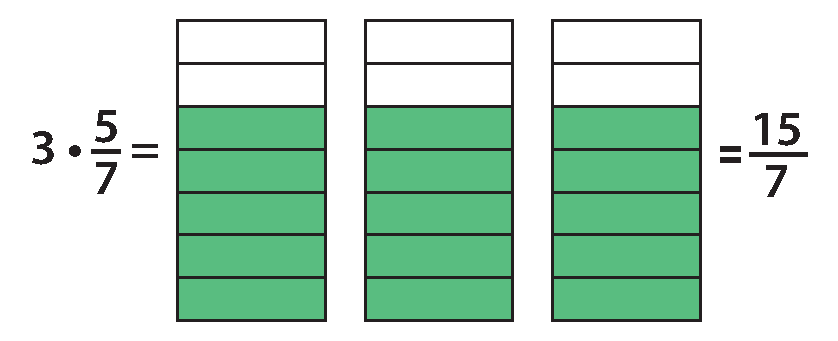
\includegraphics[scale=0.4]{pictures/Kuva3-1-1.pdf}
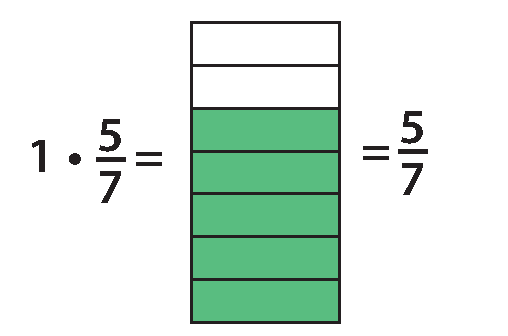
\includegraphics[scale=0.4]{pictures/Kuva3-1-2.pdf}
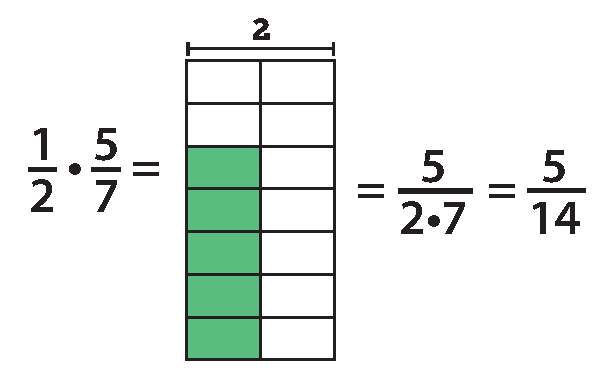
\includegraphics[scale=0.4]{pictures/Kuva3-1-3.pdf}
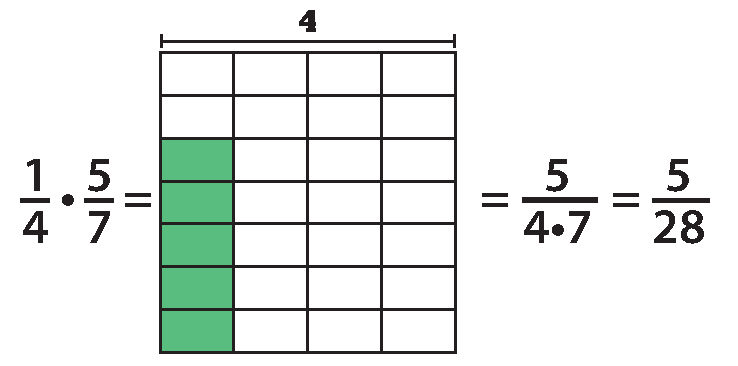
\includegraphics[scale=0.4]{pictures/Kuva3-1-4.pdf}
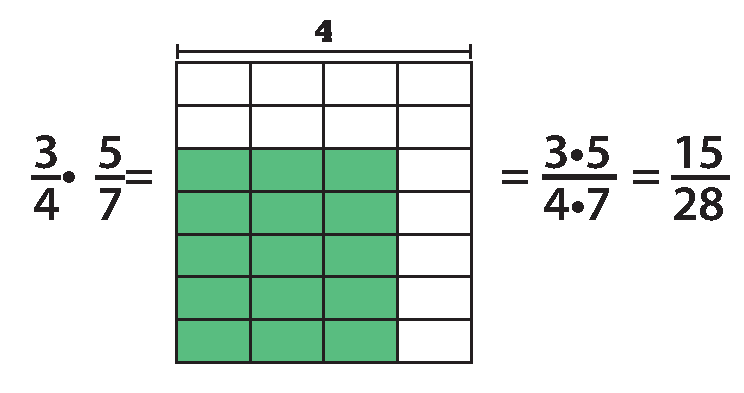
\includegraphics[scale=0.4]{pictures/Kuva3-1-5.pdf}    
    
\begin{esimerkki}
	Laske
	\[
        \frac{3}{4}\cdot \frac{6}{5}.
        \]
	
        \begin{esimratk}
        Murtolukujen kertolaskussa tekijöitä ei tarvitse laventaa samannimisiksi. Osoittajat kerrotaan keskenään ja nimittäjät kerrotaan keskenään:
      \[
        \frac{3}{4}\cdot \frac{6}{5}= \frac{3\cdot 6}{4\cdot 5}= \frac{18}{20}=\frac{9}{10}
        \]
        \end{esimratk}
        \begin{esimvast}
        $\frac{9}{10}$
        \end{esimvast}
    \end{esimerkki}
    


%esimerkkejä\ldots
% erityisesti esimerkki siitä, miten yhteiset supistettavat tekijät voi nähdä jo etukäteen, ja vältetään turhaa laskutyötä

\subsection{Murtolukujen jakolasku}

\laatikko[Käänteisluku]{
    Luvun $a$ \termi{käänteisluku}{käänteisluku} on sellainen luku $b$, joka kerrottuna luvulla a on yksi, $ab=1$.
    
    Rationaaliluvun $a$ käänteisluku on $\frac{1}{a}$ ($a\neq 0$), sillä
    \[
    a\cdot \frac{1}{a} = 1.
    \]
    Vastaavasti rationaaliluvun $\frac{a}{b}$ käänteisluku on $\frac{b}{a}$ ($a\neq 0$ ja $b\neq 0$), sillä
    \[
    \frac{a}{b}\cdot \frac{b}{a} = 1.
    \]    
%esitä analogia a-b=a+(-b) ja PERUSTELLAAN TÄLLÄ JA OSITTELULAILLA YHTEENLASKU NIMITTÄJÄSSÄ!

  %  Murtolukujen $p=\frac{a}{b}$ ja $q=\frac{c}{d}\neq 0$ \termi{osamäärä}{osamäärä} $p : q$ saadaan, kun kerrotaan luku $p$ luvun $q$ käänteisluvulla,
 %   \[
 %\frac{p}{q} = p\cdot q^{-1} = \frac{a}{b}\cdot\Big(\frac{c}{d}\Big)^{-1} = \frac{a}{b}\cdot \frac{d}{c}
 %   = \frac{ad}{bc}.
 %  \]
 }

\begin{esimerkki}
	Luvun $5$ käänteisluku on $\frac{1}{5}$, koska
	\[
	 5\cdot \frac{1}{5}=1.
	\]
	Vastaavasti luvun $-\frac{2}{3}$ käänteisluku on $-\frac{3}{2}$, koska
	\[
	 -\frac{2}{3}\cdot (-\frac{3}{2})=1.
	\]
\end{esimerkki}
  
Käänteislukua tarvitaan muun muassa murtolukujen jakolaskuissa.
 
%\begin{esimerkki}
%Laske $\frac{3}{5}:\frac{2}{7}$.

%	\begin{esimratk}
%Jakolaskun määritelmän mukaan osamäärän tulisi olla sellainen luku, joka kerrottuna jakajalla antaa tulokseksi jaettavan. Jos merkitään laskun $\frac{3}{5}:\frac{2}{7}$ vastausta kirjaimella $x$, pitää siis olla $x \cdot \frac 2 7 = \frac 3 5$.  Tätä yhtälöä kutsutaan jakolaskun $\frac 3 5 : \frac 2 7$ \termi{jakoyhtälö}{jakoyhtälöksi.}
%
%% Jakoyhtälö-termin käyttö on tässä ongelmallista, koska yhtälöt käsitellään kirjassa vasta myöhemmin.
%
%Kerrotaan jakoyhtälön molemmat puolet luvun $\frac 2 7$ käänteisluvulla $\frac 7 2$. Koska käänteislukujen tulo on $1$, saadaan
%\[
%	\text{vasen puoli} = x \cdot \underbrace{\frac 2 7 \cdot \frac 7 2}_{= 1} = x \quad \text{ja} \quad \text{oikea puoli} = \frac 3 5 \cdot \frac 7 2.
%\]
%
%% Voisi olla selkeyden vuoksi hyvä, jos käytettäisiin tässä esim. värikoodia konkretisoimaan sitä, mistä tulee x (vasen puoli) ja mistä tulee murtolukujen tulo (oikea puoli).
%Kun yhtälön molemmat puolet kerrotaan samalla luvulla, ovat myös näin saadut luvut yhtä suuria. Siis on saatu
%\[
%	x = \frac 3 5 \cdot \frac 7 2.
%\]
%Koska $x$:llä merkittiin alkuperäistä jakolaskua, on nyt onnistuttu muuttamaan jakolasku kertolaskuksi:
%\[
%	\frac 3 5 : \frac 2 7 = \frac 3 5 \cdot \frac 7 2 = \frac{3 \cdot 7}{5 \cdot 2} = \frac{21}{10} = 2 \frac{1}{10}.
%\]
%	\end{esimratk}
%\end{esimerkki}
 
\laatikko[Murtolukujen jakolasku]{
Olkoon $b \neq 0$, $c \neq 0$ ja $d \neq 0$. Murtolukujen osamäärä $\frac a b : \frac c d$ lasketaan kertomalla jaettava jakajan käänteisluvulla:
\[
	\frac a b : \frac c d = \frac a b \cdot \frac d c = \frac{ad}{bc}.
\]
}

%vaikeampia jakolaskuesimerkkejä, kirjaimia mukaan!

\begin{esimerkki}
Jos jonkin luvun jakaminen päässä viidellä tuntuu vaikealta, voi käyttää esimerkiksi seuraavaa kikkaa: Koska $5$ vastaa arvoltaa lauseketta $10:2$, voidaan viidellä jakamisen sijaan jakaa $\frac{10}{2}$:lla. Tämä voi helpottaa päässälaskua, koska yleensä kahdella ja kymmenellä suoritetut kerto- ja jakolaskut koetaan yksinkertaisina. Jaetaan mielivaltainen $x$ viidellä näin:
$$x:5=x:\frac{10}{2}=x\cdot \frac{2}{10}=\frac{2x}{10}$$

Viidellä tulee siis jaettua, jos kertoo kahdella ja jakaa tmän jälkeen tulon kymmenellä. (Toki myös laskujärjestys $\frac{x}{10}\cdot 2$ on mahdollinen, eli että ensin jakaa kymmenellä ja sitten vasta kertoo kahdella.) Näin esimerkiksi lasku $1\,340:5$ muuttuu muotoon $\frac{1\,340\cdot 2}{10}=\frac{2\,680}{10}=268$.
\end{esimerkki}

\subsection{Murtolausekkeiden sieventäminen}

\laatikko[Yhteiseksi tekijäksi ottaminen]{
Jos murtoluvun osoittajassa tai nimittäjässä on summa, jonka osilla on yhteinen tekijä, sen voi ottaa \emph{yhteiseksi tekijäksi} sulkujen eteen. Jos osoittajassa ja nimittäjässä on sen jälkeen sama kerroin, sen voi jakaa pois molemmista eli \emph{supistaa} pois.
\begin{equation}
\frac{ac+bc}{c} = \frac{ \cancel{c} (a+b)}{\cancel{c}} = a+b
\end{equation}

Joskus murtolauseke sieventyy, jos sen esittääkin kahden murtoluvun summana.
\begin{equation}
\frac{ca+b}{c} = \frac{ca}{c} + \frac{b}{c} = a + \frac{b}{c}
\end{equation}
}

\begin{esimerkki}
Kun jakaa kolme erikokoista nallekarkkipussia ($a$, $b$ ja $c$) tasan kolmen ihmisen kesken, on sama, laittaako kaikki ensin samaan kulhoon ja jakaa ne sitten ($\frac{a+b+c}{3}$) vai jakaako jokaisen pussin erikseen ($ \frac{a}{3} + \frac{b}{3} + \frac{c}{3}$).

Jos taas samat kolme henkilöä jakavat keskenään pussin tikkareita ($6$ kpl) ja yhden pussin nallekarkkeja ($n$ kpl), niin saadaan seuraavanlainen lasku: $ \frac{6\text{ tikkaria}+n\text{ nallekarkkia}}{3} = \frac{6\text{ tikkaria}}{3} + \frac{n\text{ nallekarkkia}}{3} = \frac{\cancel{3} \cdot 2\text{ tikkaria}}{\cancel{3}} + \frac{n\text{ nallekarkkia}}{3} = 2\text{ tikkaria} + \frac{n\text{ nallekarkkia}}{3}$. Toisin sanoen, kukin saa kaksi tikkaria ja kuinka paljon ikinä onkaan kolmasosa kaikista nallekarkeista.
\end{esimerkki}

%tarviataanko? tehtäviä on.
%\laatikko[Ryhmittely]{
%Samantyyppiset asiat voidaan laskea yhteen tai \emph{ryhmitellä}.
%\begin{equation}
%ax^2 + bx + cx^2 + dy + ex = (a+c)x^2 + (b+e)x + dy
%\end{equation}
%}